\documentclass{beamer}
\usepackage[utf8]{inputenc}
\usepackage[T1]{fontenc}
\usepackage[spanish,es-noshorthands]{babel}
\usepackage{lmodern}
\usepackage{graphicx}
\usepackage{booktabs}
\usepackage{amsmath}
\usepackage{amssymb}
\usepackage{tikz}
\usetikzlibrary{positioning, arrows.meta, calc}

\usetheme{Madrid}
\usecolortheme{default}

\title{Control STR del Péndulo Invertido}
\subtitle{Self-Tuning Regulator adaptativo indirecto en tiempo discreto}
\author{Lucas Gaggino}
\institute{Facultad de Ingeniería - UBA \\ Control Adaptativo 86.20}

\begin{document}

\begin{frame}
\titlepage
\end{frame}

\begin{frame}{Contenido}
\tableofcontents
\end{frame}

% ==================================================================
\section{El Sistema}
% ==================================================================

\begin{frame}{Sistema del Péndulo Invertido}
\begin{block}{Ecuación No Lineal}
\[
(M + m)\ddot{x} = F - ml\ddot{\theta}\cos\theta + ml\dot{\theta}^2\sin\theta
\]
\[
ml\ddot{\theta}\cos\theta + ml\dot{\theta}^2\sin\theta + mg\sin\theta = 0
\]
\end{block}
\begin{block}{Modelo Linealizado ($\theta = 0$, inestable)}
\[
\ddot{\theta} = A_\theta\theta + B_\theta F, \qquad
A_\theta = 15{,}79, \quad B_\theta = -1{,}4634
\]
El signo $B_\theta < 0$ es físico: $F>0$ reduce $\theta$.
\end{block}
\end{frame}

\begin{frame}{Discretización ZOH analítica $\rightarrow$ modelo ARX}
\begin{block}{Sin pasar por tiempo continuo}
Para $G(s) = B_\theta/(s^2 - w^2)$, $w = \sqrt{A_\theta}$, con $T_s = 0{,}02$~s:
\[
A(z) = z^2 - 2\cosh(wT_s)z + 1, \quad
B(z) \propto (z+1)
\]
\[
G(z) = \frac{-2{,}93\times10^{-4}\,(z+1)}{z^2 - 2{,}0063\,z + 1}
\]
\end{block}
\begin{block}{Características}
\begin{itemize}
  \item Polo inestable en $z \approx 1{,}083$; polo estable en $z \approx 0{,}924$.
  \item Cero en $z \approx -1$: \textbf{no de fase mínima} $\Rightarrow$ no se cancela.
\end{itemize}
\end{block}
\end{frame}

% ==================================================================
\section{Método STR}
% ==================================================================

\begin{frame}{¿Por qué STR y todo en discreto?}
\begin{itemize}
  \item \textbf{Self-Tuning Regulator (STR)}: estima la planta on-line y
  rediseña el controlador automáticamente (autoajuste).
  \item \textbf{Indirecto}: RLS estima $A(q),B(q)$; luego se diseña por
  \emph{certainty equivalence}.
  \item \textbf{Todo discreto}: el regulador se obtiene resolviendo la ecuación
  Diofantina en $q^{-1}$, sin conversión a continuo (Tustin) como antes.
\end{itemize}
\begin{block}{Ley de control RST (2 grados de libertad)}
\[
R(q)\,u_k = T(q)\,r_k - S(q)\,y_k
\]
\end{block}
\end{frame}

\begin{frame}{Colocación de polos: ecuación Diofantina}
\begin{block}{Identidad de Bézout}
\[
A(q)\,R(q) + B(q)\,S(q) = A_{lc}(q)
\]
Se resuelve armando la \textbf{matriz de Sylvester} (Toeplitz de $A$ y $B$).
\end{block}
\begin{block}{Rechazo de perturbaciones (teoría STR)}
\[
y = \frac{BT}{AR+BS}\,r + \frac{BR}{AR+BS}\,v
\]
\begin{itemize}
  \item Perturbación escalón $\Rightarrow$ $R$ debe tener raíz en $z=1$
  (integrador $1-q^{-1}$).
  \item Ruido de medición $\Rightarrow$ RLS lo filtra.
\end{itemize}
\end{block}
\end{frame}

\begin{frame}{Estimación RLS con olvido}
\begin{block}{Modelo ARX y actualización recursiva}
\[
\epsilon(k) = y(k) - \varphi^\top(k)\hat\theta(k-1)
\]
\[
K(k) = \frac{P\varphi}{\lambda + \varphi^\top P\varphi}, \quad
\hat\theta(k) = \hat\theta(k-1) + K(k)\epsilon(k)
\]
\[
P(k) = \tfrac{1}{\lambda}(I - K\varphi^\top)P(k-1)
\]
\end{block}
Regresor: $\varphi = [-y_{k-1}, -y_{k-2}, u_{k-1}, u_{k-2}]$,
$\ \hat\theta = [a_1,a_2,b_1,b_2]$, $\lambda = 0{,}995$.
\end{frame}

% ==================================================================
\section{Diseño del Regulador}
% ==================================================================

\begin{frame}{Diseño discreto: pasos}
\begin{enumerate}
  \item \textbf{Integrador}: diseñar sobre $\bar A = A(1-q^{-1})$ (grado 3),
  luego $R = (1-q^{-1})\bar R$.
  \item \textbf{Polos LC}: mapear $\{-3,-3,-10\}$ con $z=e^{sT_s}$
  $\rightarrow \{0{,}942,\ 0{,}942,\ 0{,}819\}$ + 2 auxiliares en $0{,}2$
  (grado 5).
  \item \textbf{Sin cancelación} del cero en $z\approx-1$.
  \item \textbf{Sylvester} $\Rightarrow R,S$ de mínimo orden
  ($\deg S = \deg \bar A - 1 = 2$).
  \item \textbf{Feedforward}: $t_0 = A_{lc}(1)/B(1)$ (ganancia estática unitaria).
\end{enumerate}
\begin{block}{Regulador nominal resultante}
\[
R = [1, -1{,}20,\ 0{,}23,\ -0{,}03], \quad
S = [-366{,}8,\ 697{,}2,\ -331{,}1], \quad t_0 = -0{,}67
\]
\end{block}
\end{frame}

\begin{frame}{Estructura RST}
\begin{figure}
\centering
\begin{tikzpicture}[>=Latex, node distance=1.2cm, auto,
  block/.style={draw, rectangle, minimum height=0.9cm, minimum width=1.4cm, align=center},
  sum/.style={draw, circle, inner sep=0pt, minimum size=6mm}]
  \node (r) {$r_k$};
  \node[block, right=1.0cm of r] (T) {$\dfrac{T}{R}$};
  \node[sum, right=1.0cm of T] (s1) {$+$};
  \node[block, right=1.0cm of s1] (P) {$\dfrac{B}{A}$};
  \node[right=1.3cm of P] (y) {$y_k$};
  \node[block, below=1.0cm of s1] (S) {$\dfrac{S}{R}$};
  \draw[->] (r) -- (T);
  \draw[->] (T) -- (s1);
  \draw[->] (s1) -- node {$u_k$} (P);
  \draw[->] (P) -- (y);
  \draw[->] ($(P)!0.5!(y)$) |- (S);
  \draw[->] (S) -| node[pos=0.95, left] {$-$} (s1);
\end{tikzpicture}
\end{figure}
\begin{block}{Algoritmo adaptativo indirecto}
En cada $k$: RLS $\rightarrow \hat A,\hat B$; cada $N$ pasos rediseño RST
(Diofantina); aplicar $u_k$; integrar planta no lineal (ZOH).
\end{block}
\end{frame}

% ==================================================================
\section{Resultados}
% ==================================================================

\begin{frame}{Mapa de polos y ceros discreto}
\begin{center}
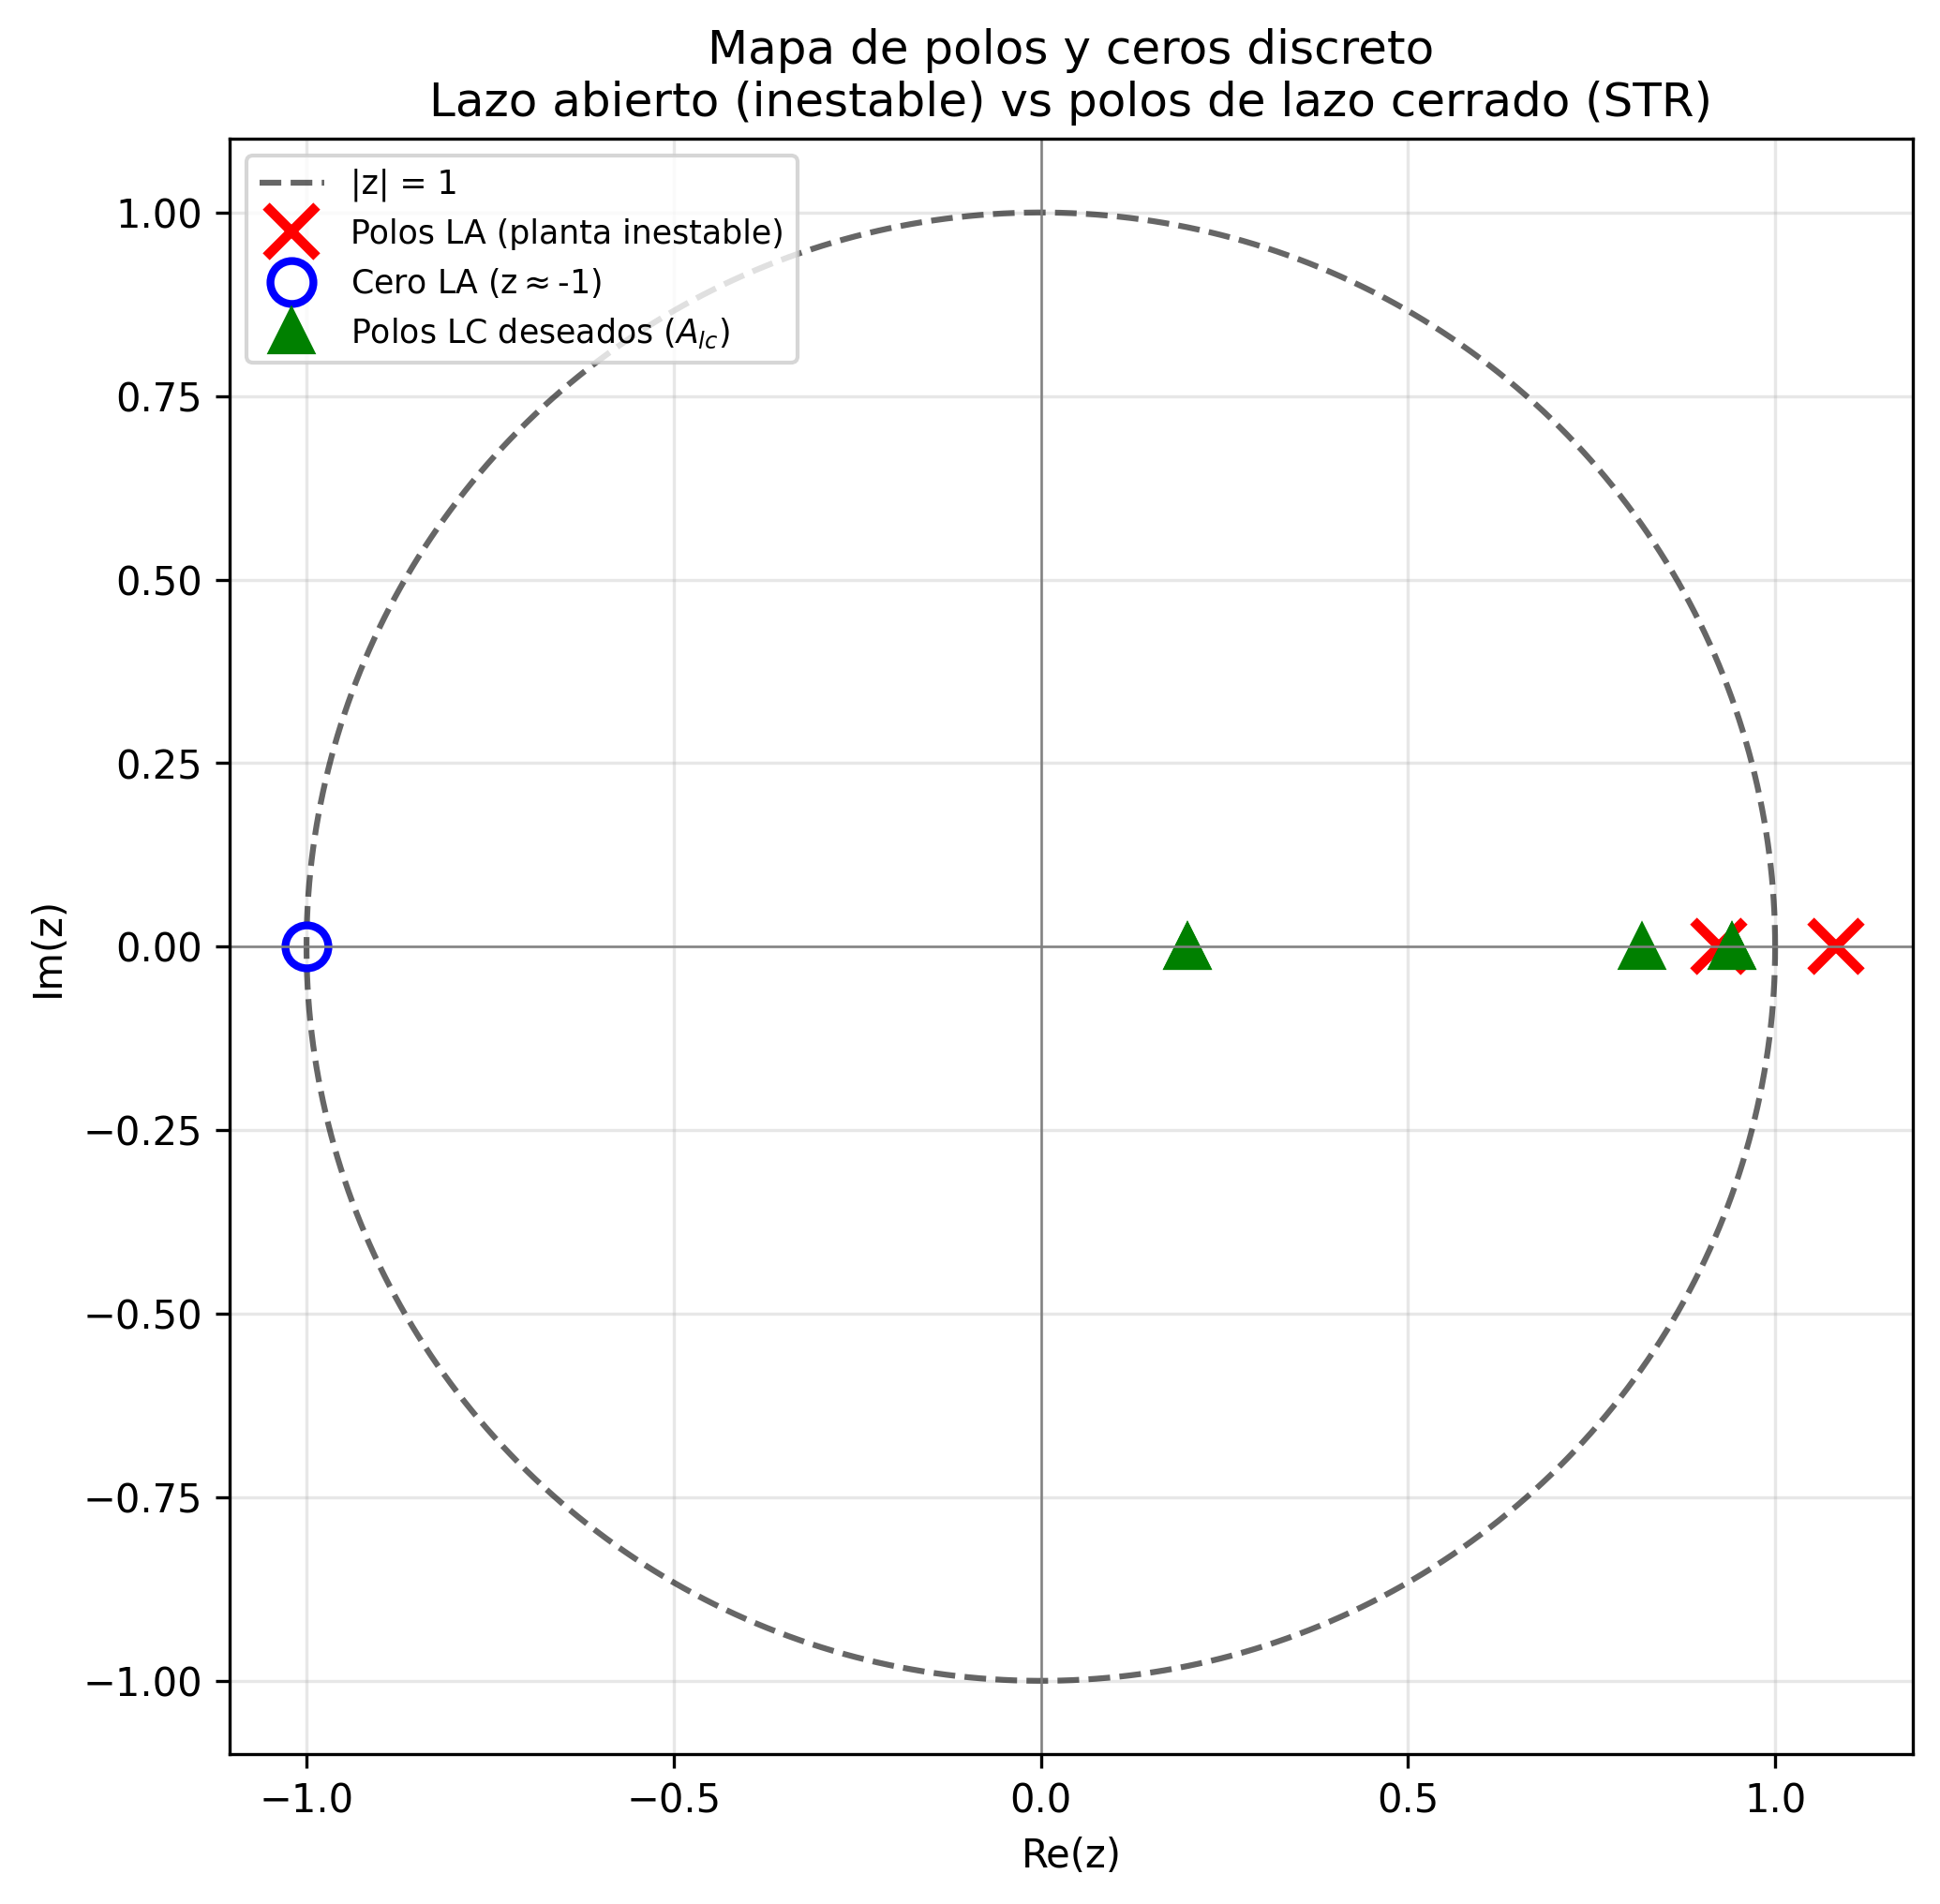
\includegraphics[width=0.62\textwidth]{imagenes_pid_autotunning/str_polos_ceros.png}
\end{center}
El STR mueve los polos dentro del círculo unitario sin cancelar el cero en
$z\approx-1$.
\end{frame}

\begin{frame}{Resultados: sin perturbaciones}
\begin{center}
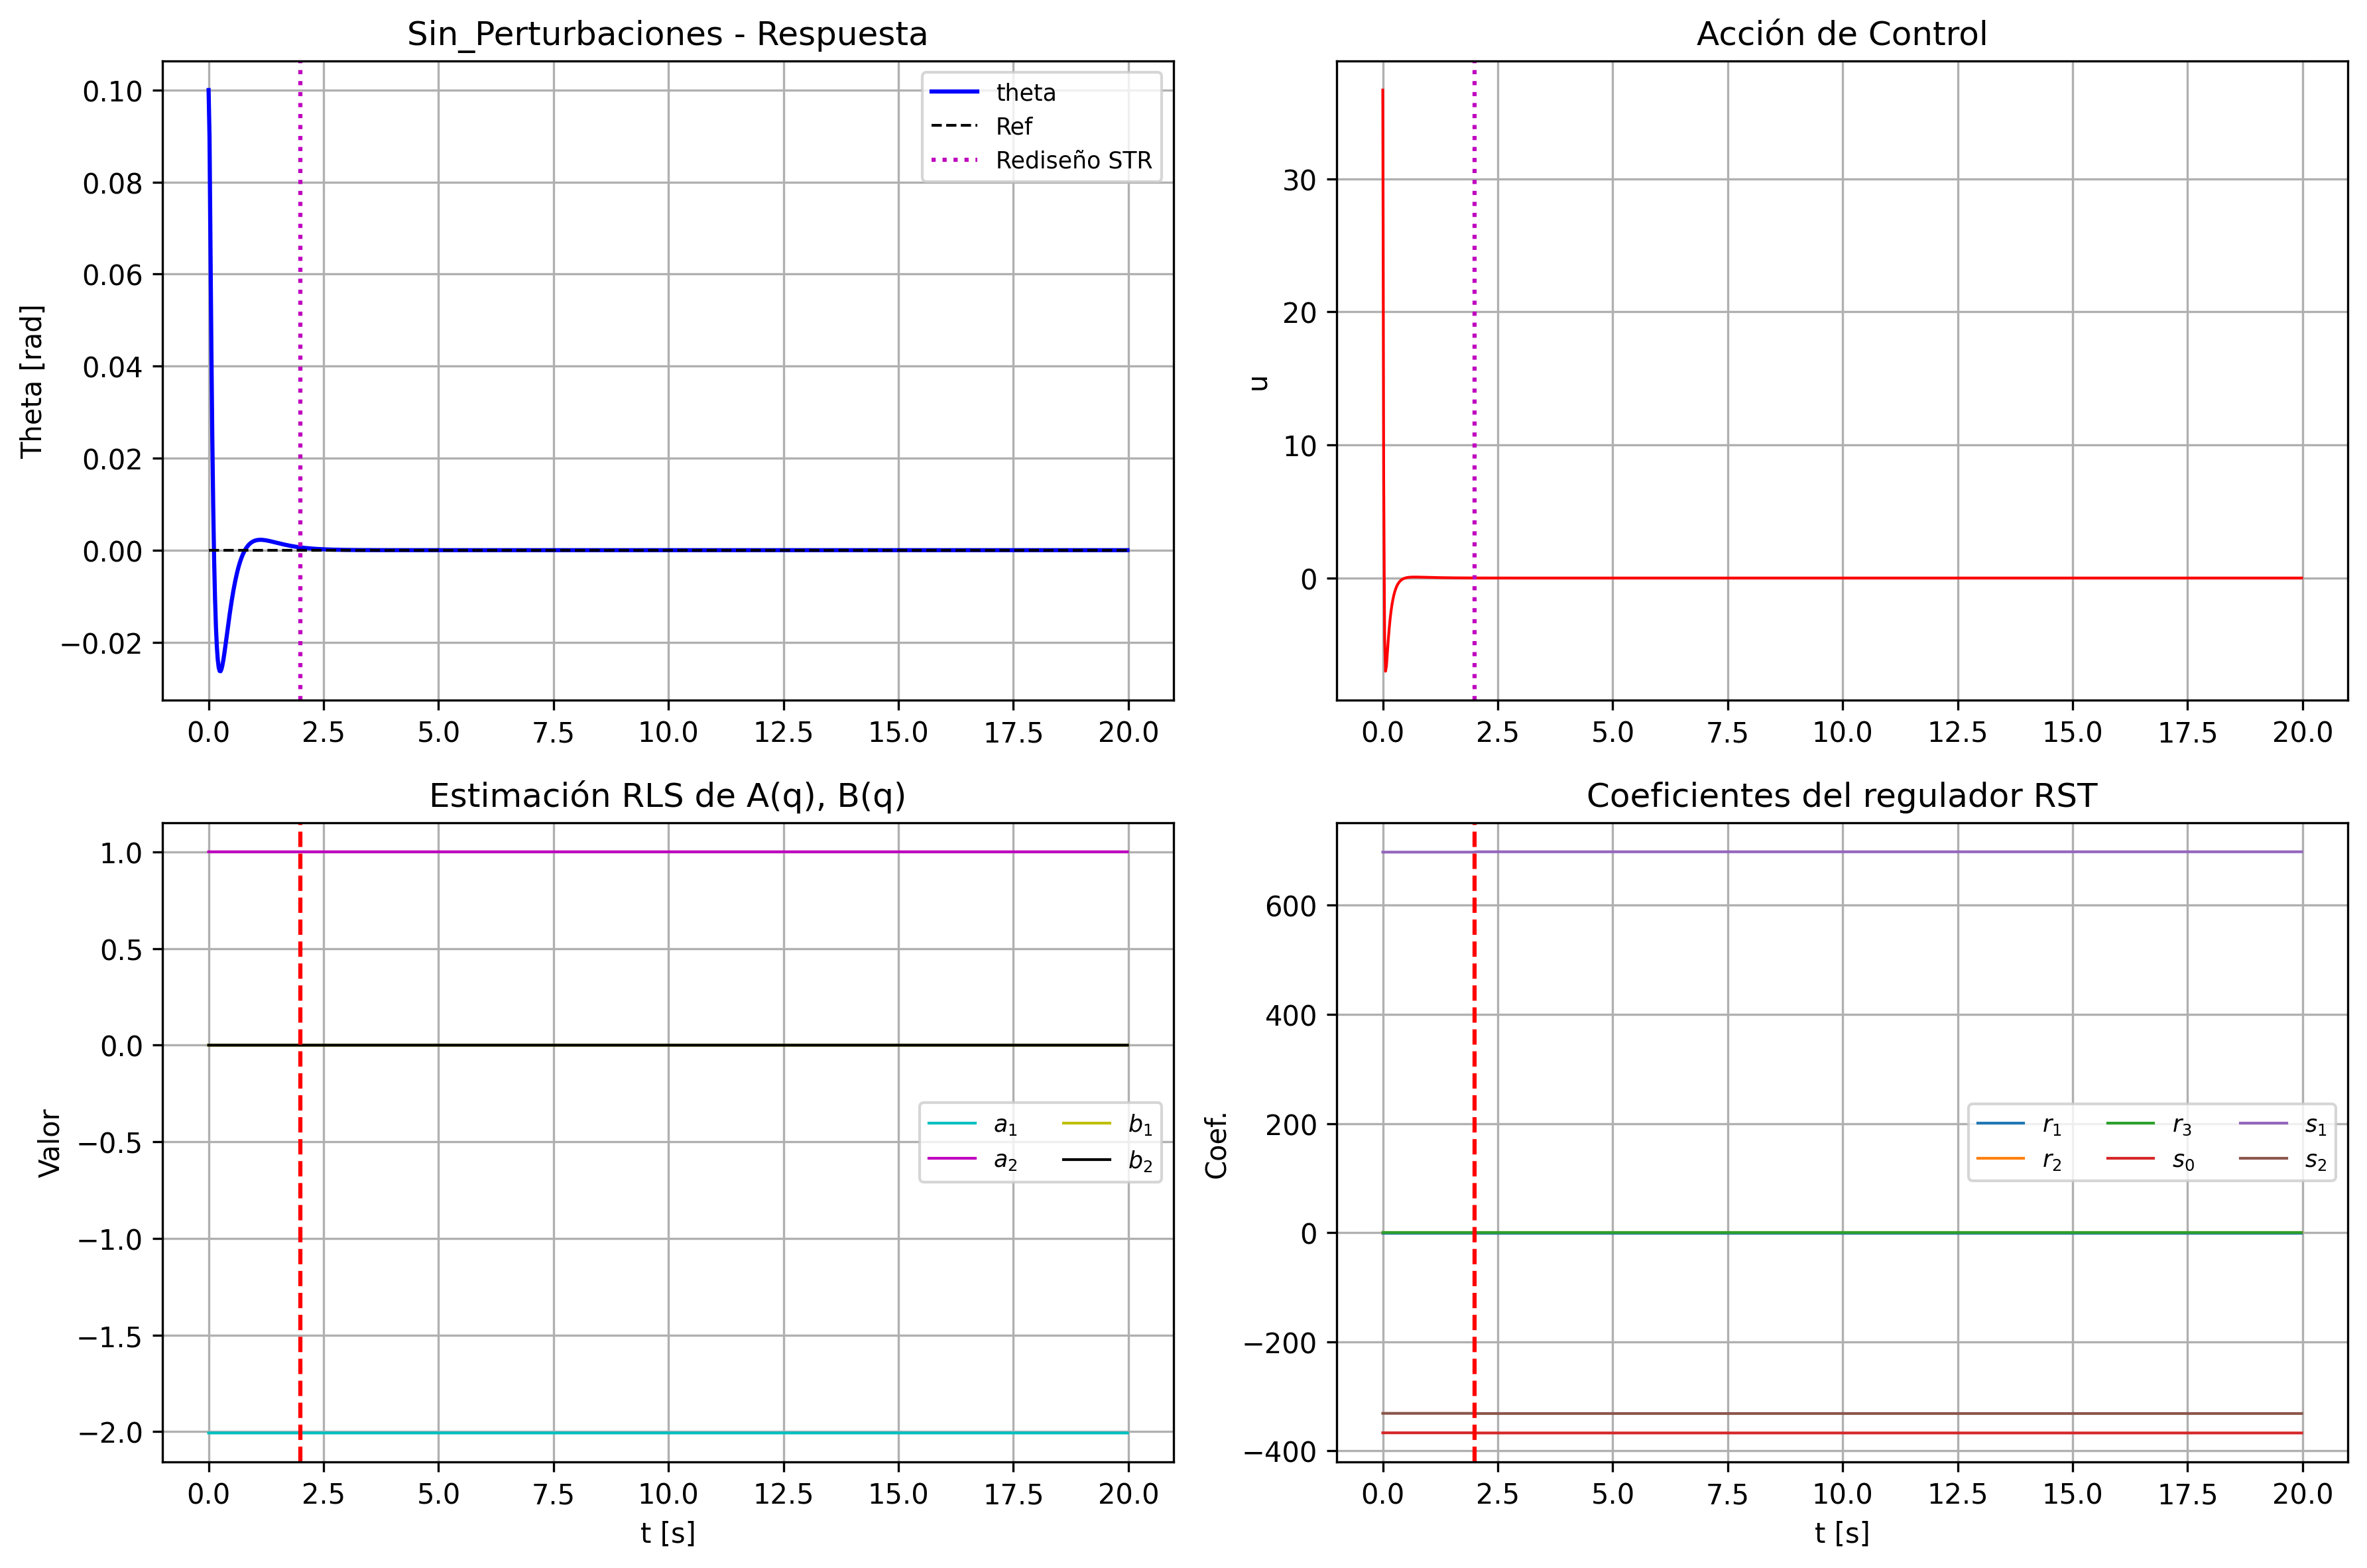
\includegraphics[width=0.9\textwidth]{imagenes_pid_autotunning/str_Sin_Perturbaciones.png}
\end{center}
Estabilización desde $\theta(0)=0{,}1$; RLS converge a los valores reales.
\end{frame}

\begin{frame}{Resultados: perturbación sinusoidal}
\begin{center}
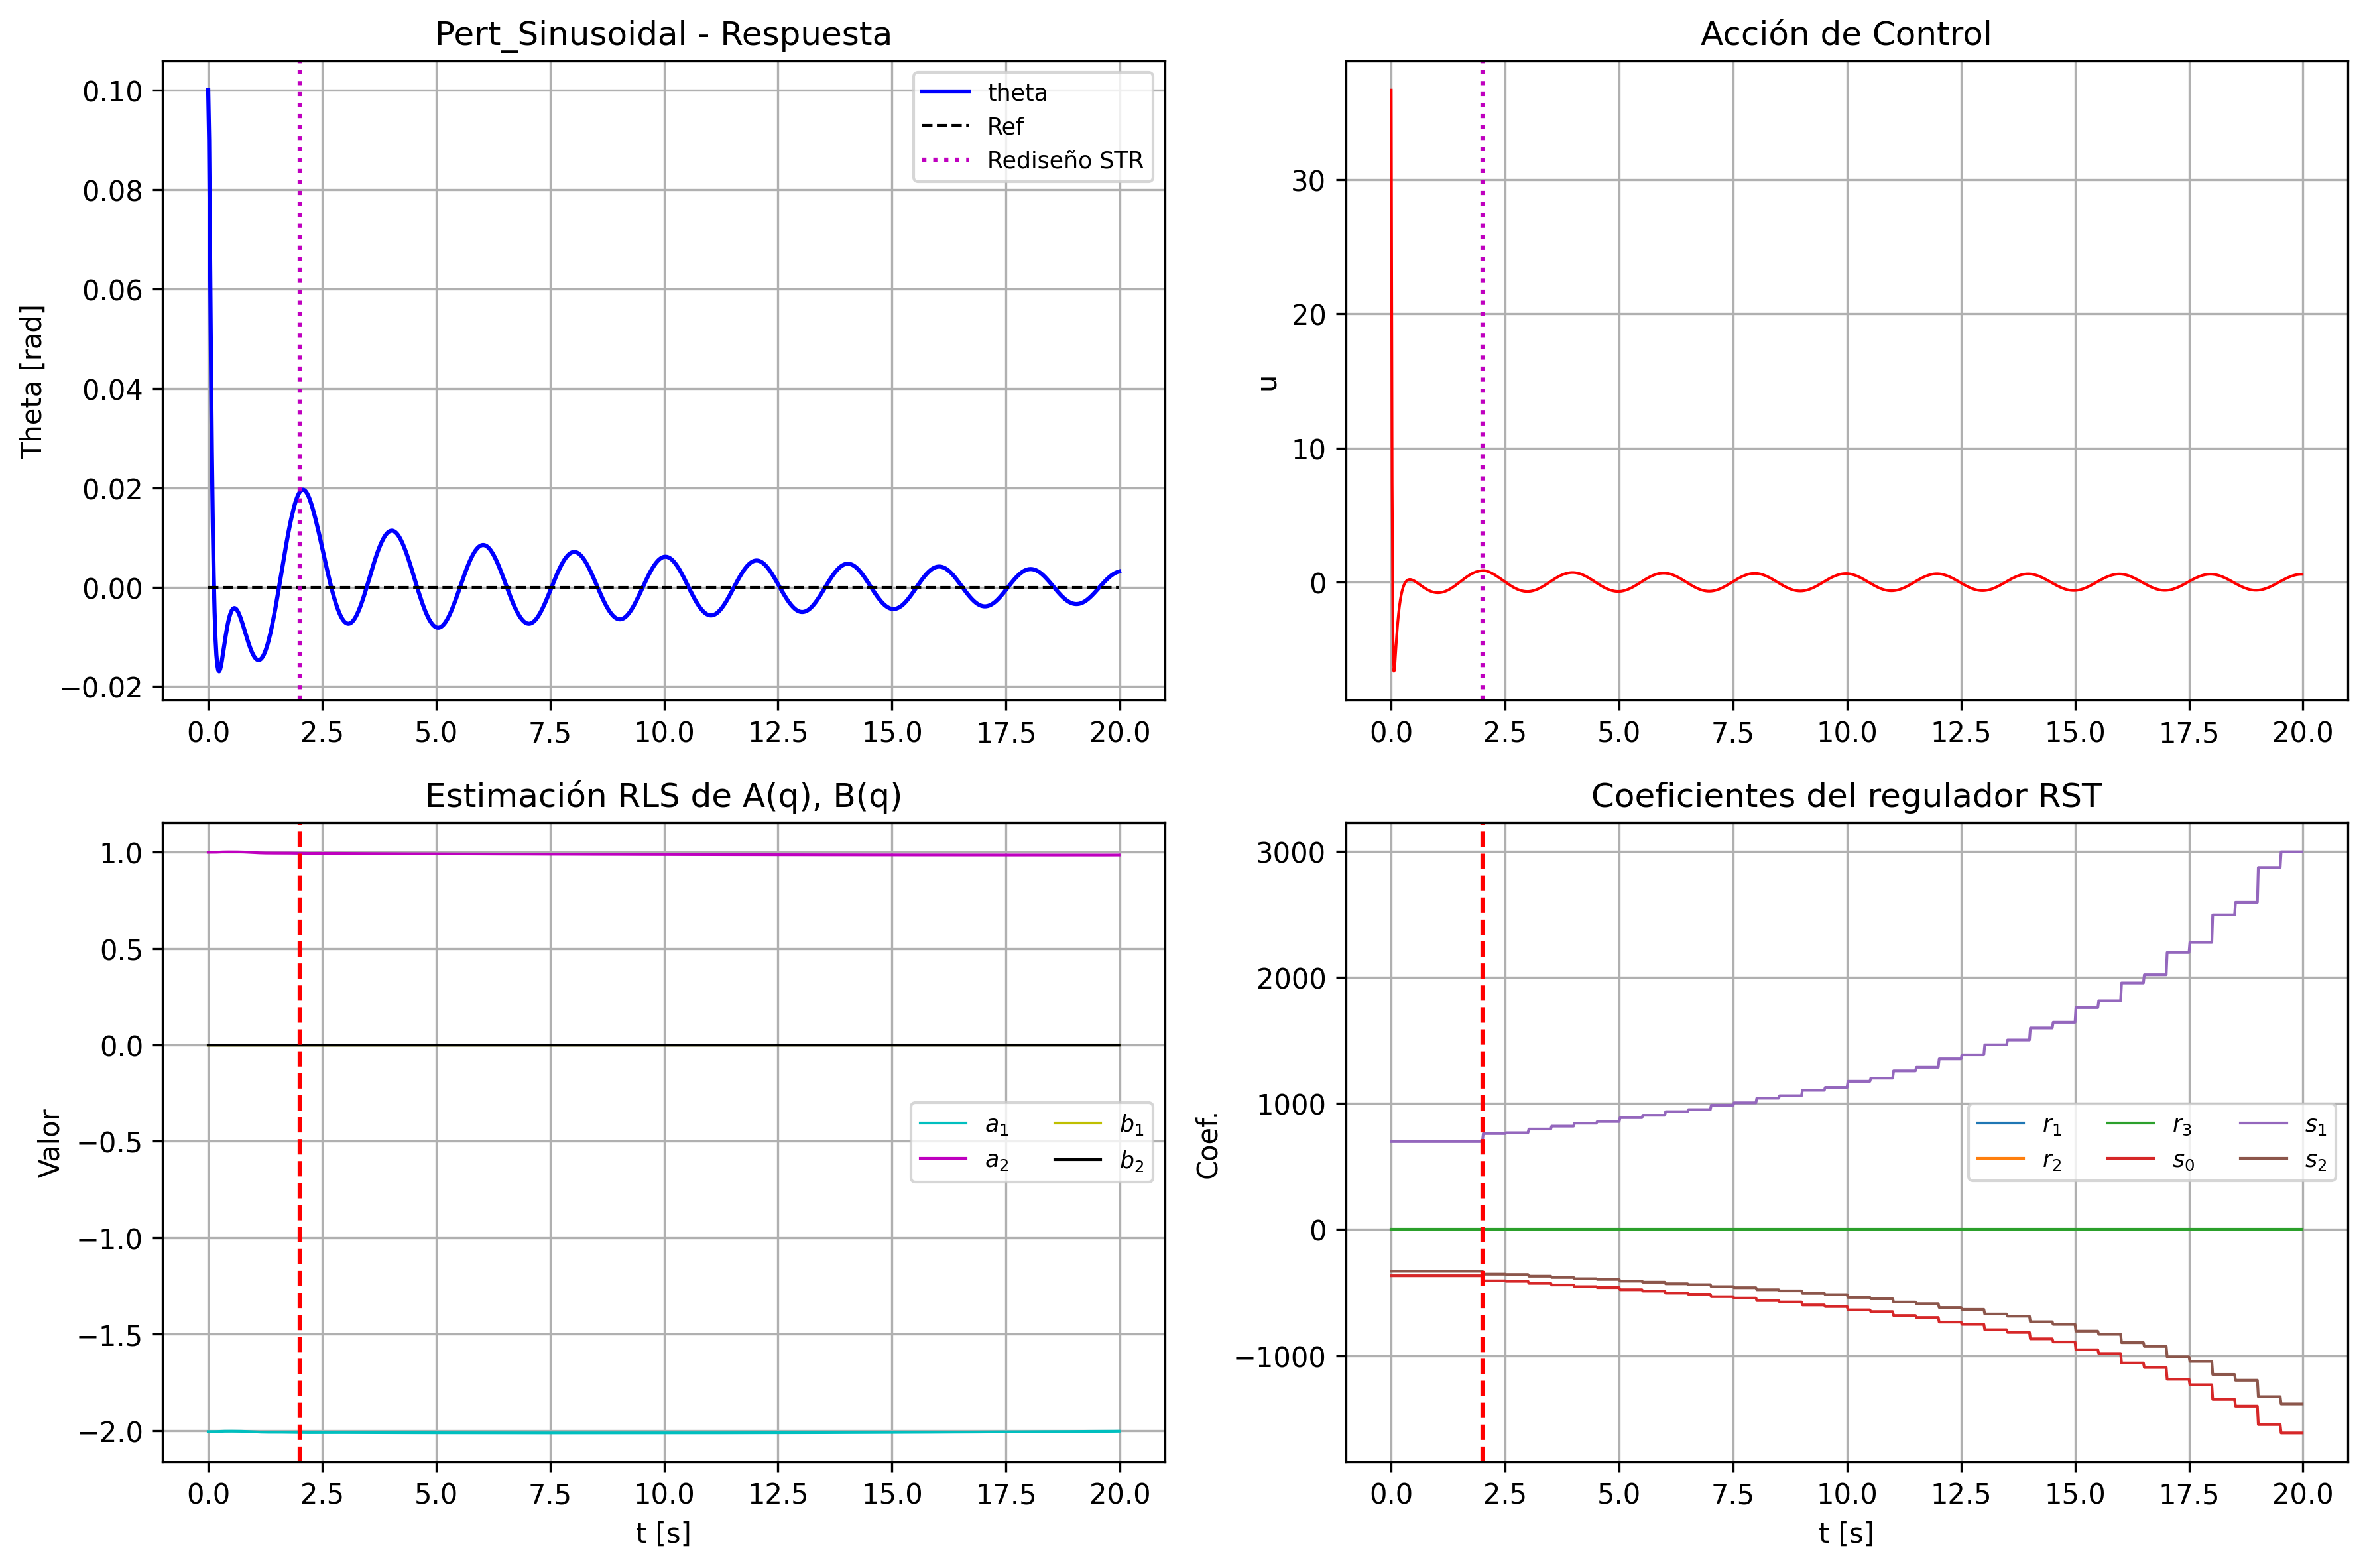
\includegraphics[width=0.9\textwidth]{imagenes_pid_autotunning/str_Pert_Sinusoidal.png}
\end{center}
\end{frame}

\begin{frame}{Resultados: perturbación escalón}
\begin{center}
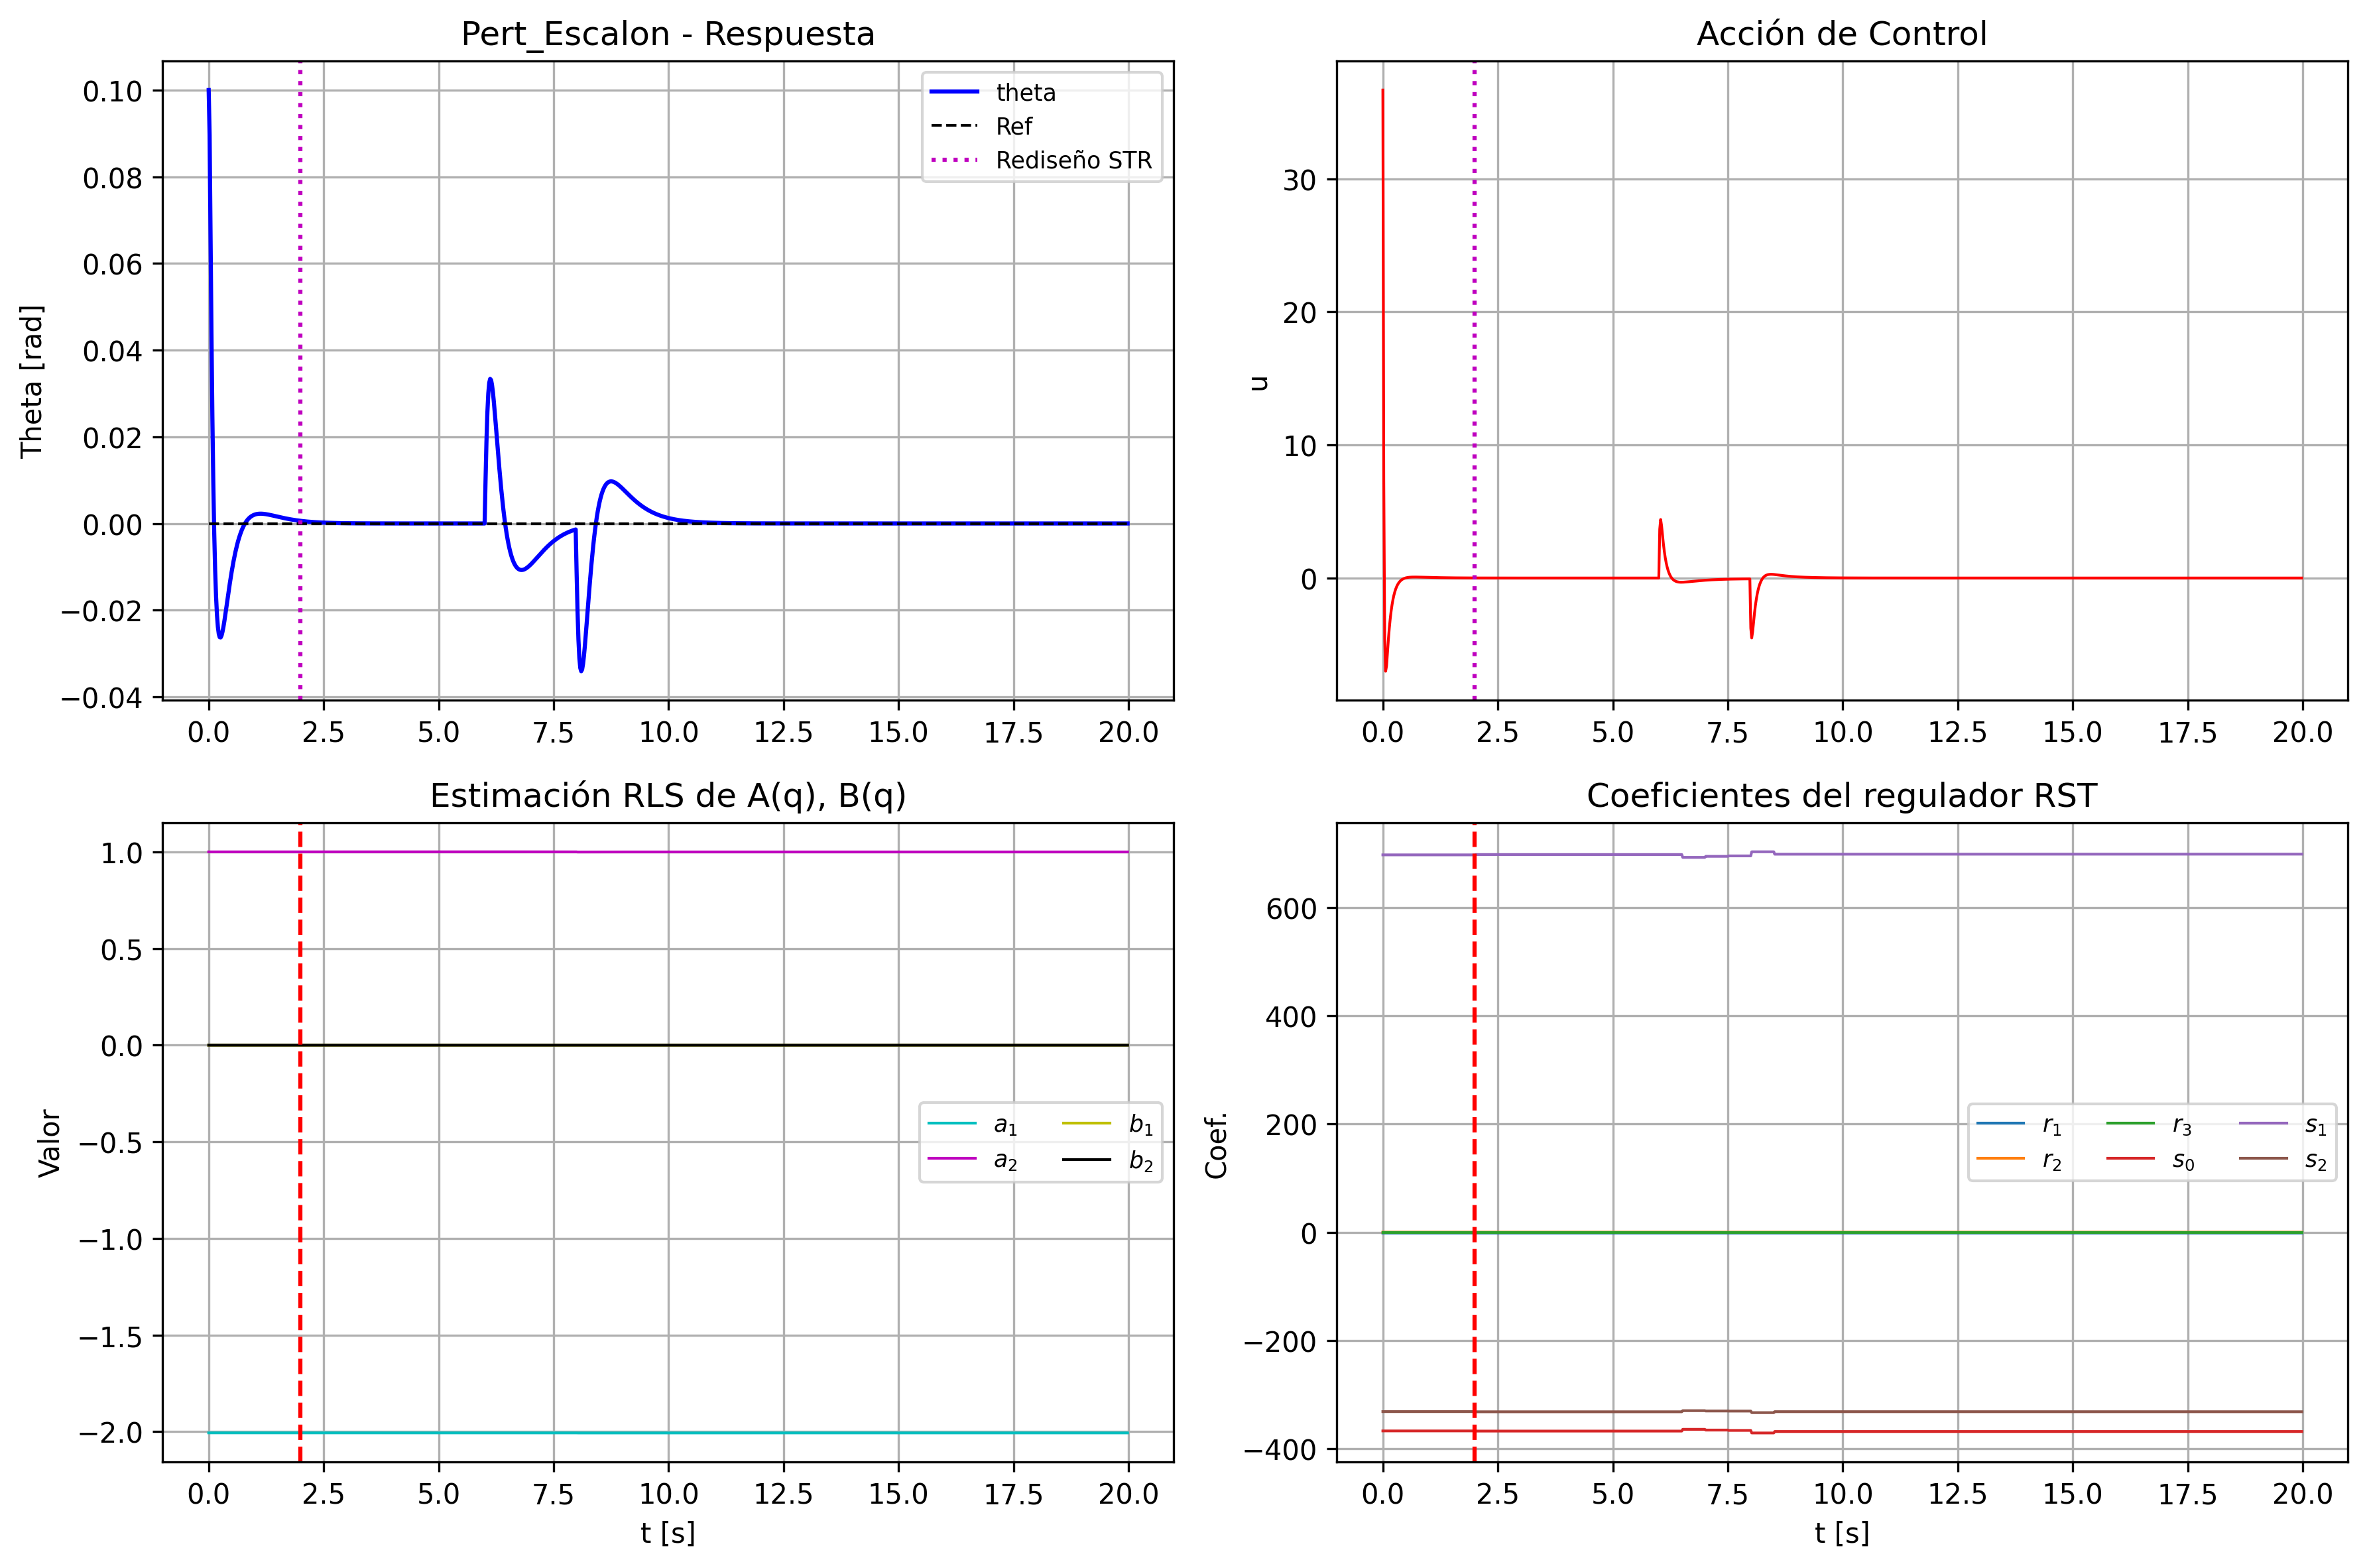
\includegraphics[width=0.9\textwidth]{imagenes_pid_autotunning/str_Pert_Escalon.png}
\end{center}
El integrador $(1-q^{-1})$ en $R$ rechaza la perturbación escalón.
\end{frame}

\begin{frame}{Resultados: ruido de medición}
\begin{center}
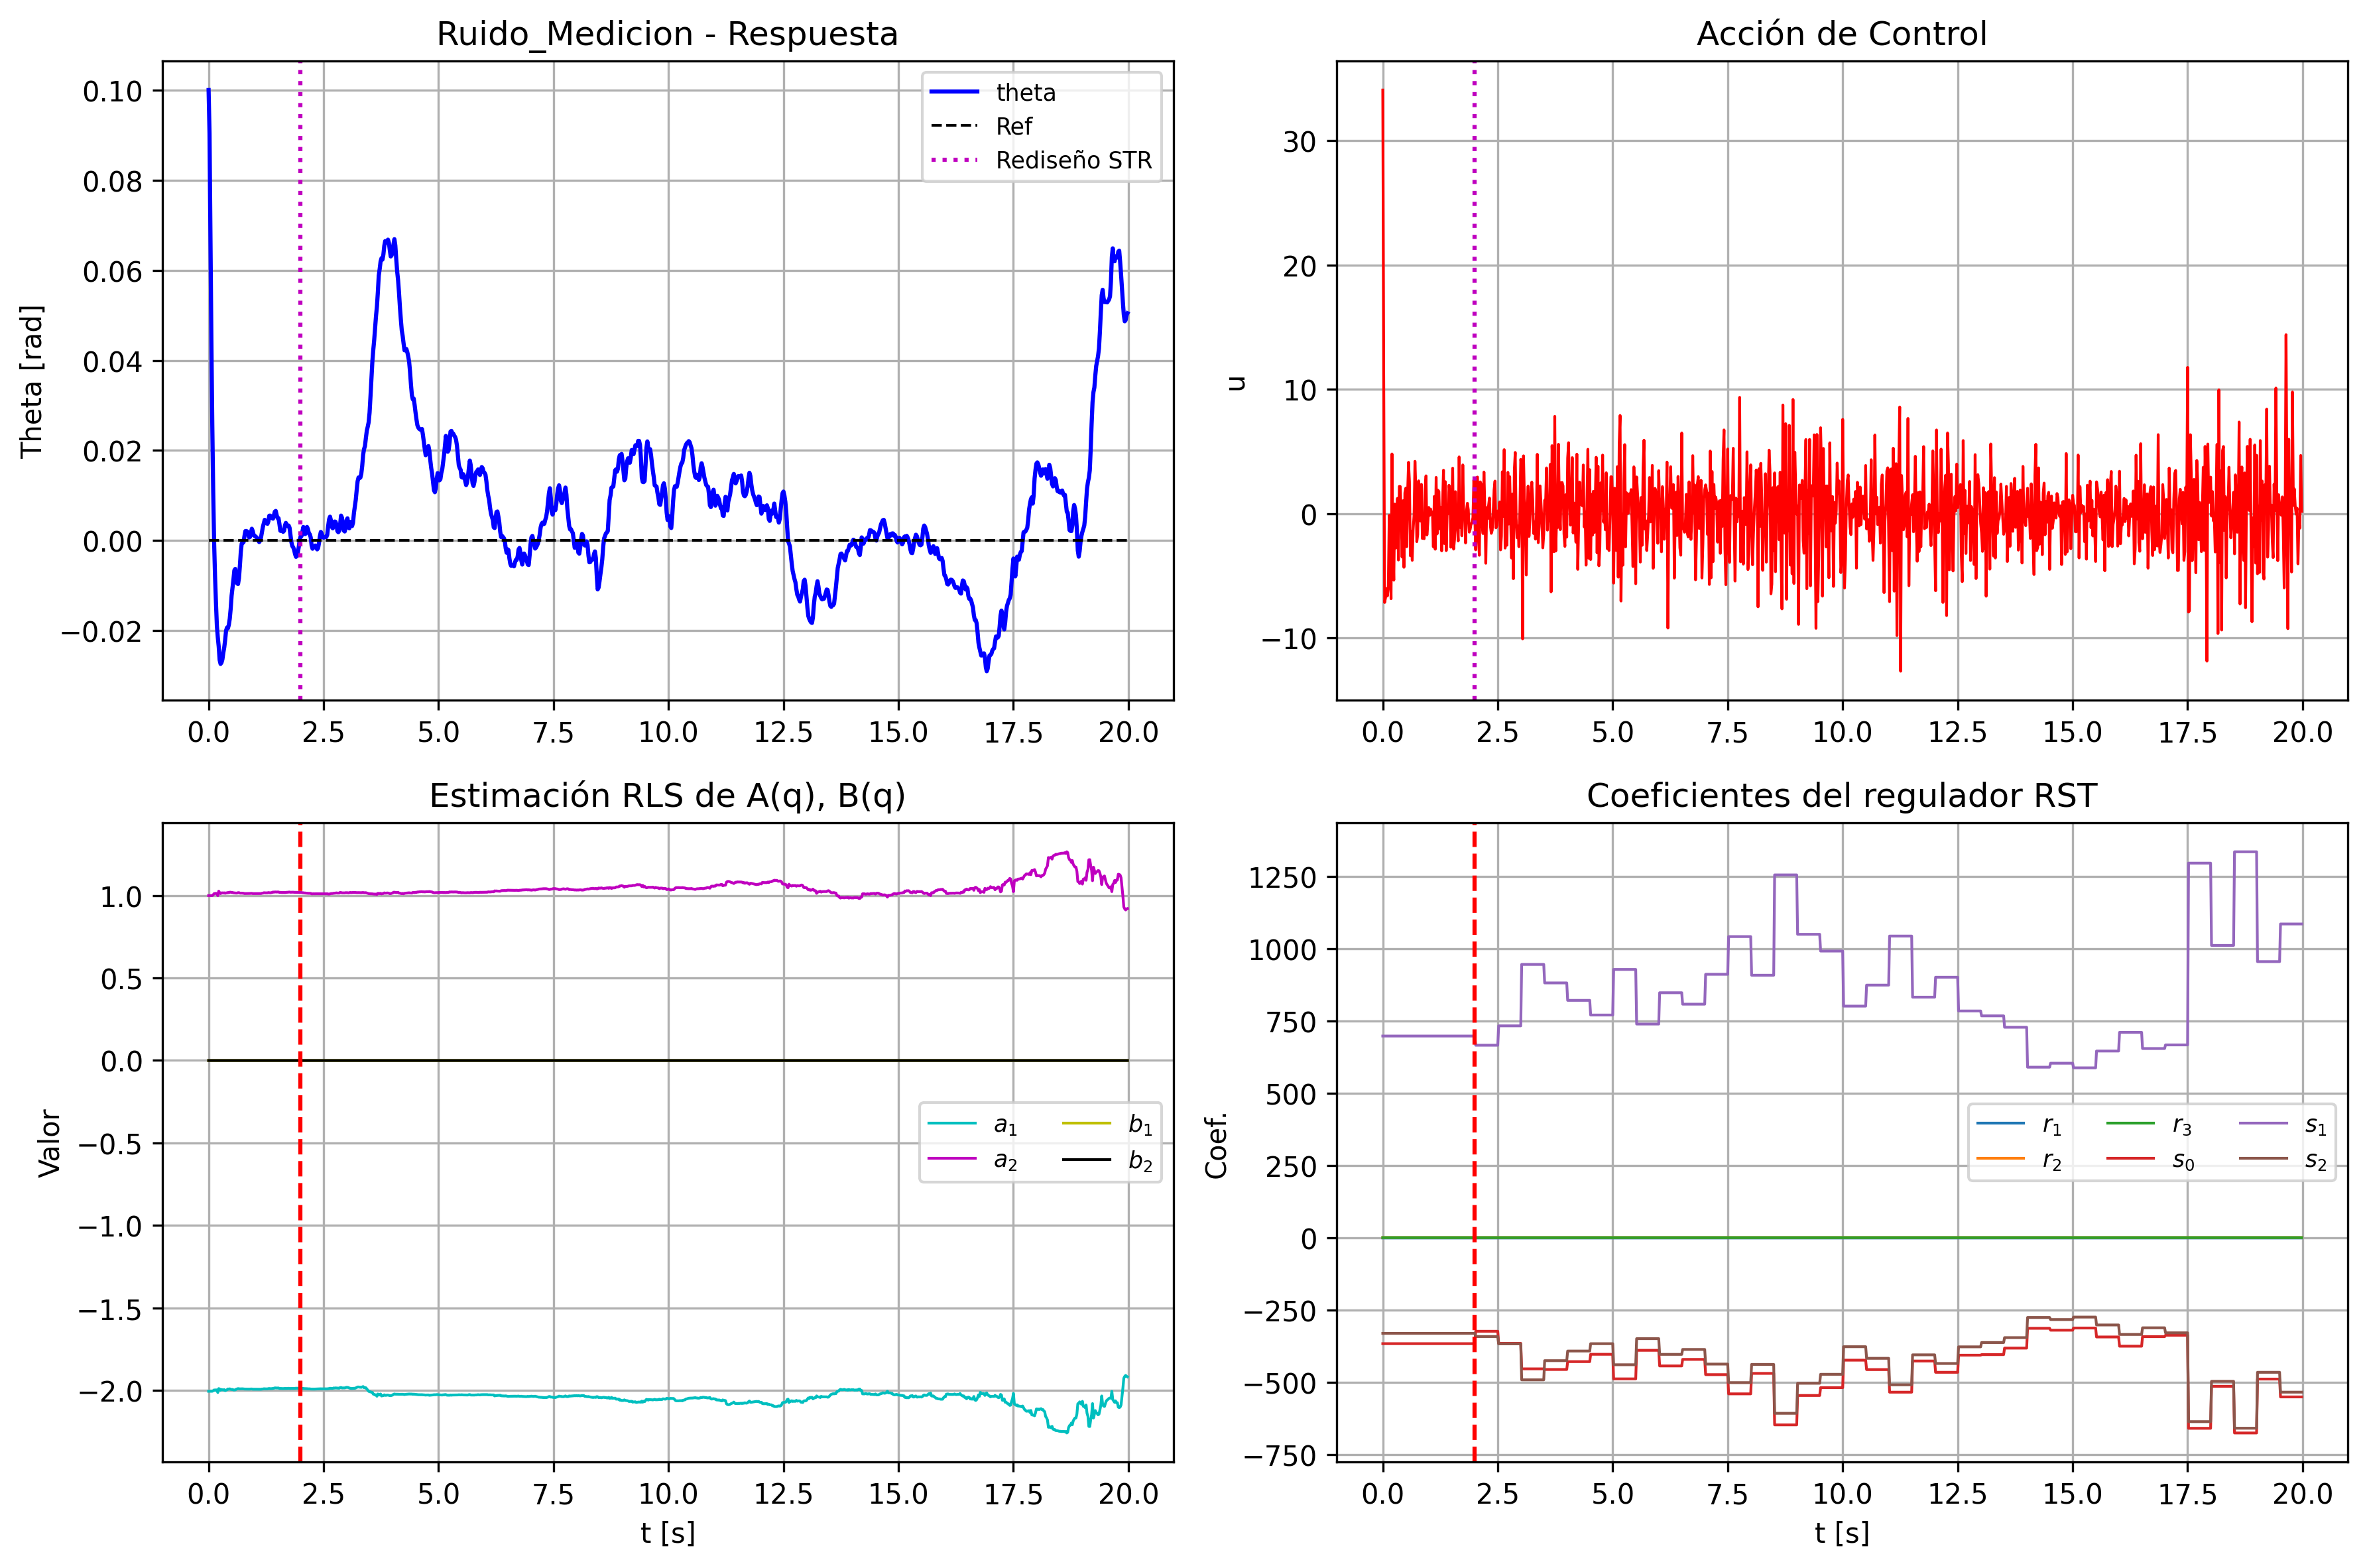
\includegraphics[width=0.9\textwidth]{imagenes_pid_autotunning/str_Ruido_Medicion.png}
\end{center}
El lazo es estable, pero el regulador \textbf{no converge} (persigue el ruido).
\end{frame}

% ==================================================================
\section{Convergencia y robustez}
% ==================================================================

\begin{frame}{¿Por qué $R,S,T$ no convergen con ruido/sinusoidal?}
\begin{itemize}
  \item El lazo es \textbf{estable} en los 4 casos ($\theta$ acotado), pero
  $R,S,T$ \textbf{no convergen} con ruido ni perturbación sinusoidal.
  \item Causa raíz: el numerador $B$ es diminuto ($b_1{+}b_2\approx-5{,}9\times10^{-4}$)
  y va al \textbf{denominador} del diseño ($t_0=A_{lc}(1)/B(1)$, Sylvester).
  \item Un pequeño error en $b$ (por ruido o \emph{covariance windup}) se
  amplifica: $b_1$ cambia de signo, $s_0$ crece $\sim4\times$ y deriva.
  \item Consecuencia: los polos logrados \emph{sobre la planta real} se corren al
  borde ($0{,}989$--$0{,}995$), perdiendo margen.
\end{itemize}
\end{frame}

\begin{frame}{Variante robusta (comparable con la básica)}
\begin{block}{Mejoras (flag \texttt{robust})}
\begin{itemize}
  \item Regresor consistente con la salida medida.
  \item \textbf{Zona muerta} en RLS ($\sim\sigma\lVert[1,a_1,a_2]\rVert$): no
  adapta sobre ruido/perturbación puros.
  \item Anti \emph{windup} de covarianza (acota $\mathrm{tr}(P)$).
  \item \textbf{Gate} de rediseño validado contra el prior nominal confiable
  (signo/magnitud de $b$, $\lVert S\rVert$, estabilidad) + congelamiento.
\end{itemize}
\end{block}
Resultado: $R,S,T$ convergen y se recuperan \textbf{exactamente} los polos de
diseño ($\max|z|=0{,}9418$) en los 4 escenarios.
\end{frame}

\begin{frame}{Comparación: convergencia del regulador}
\begin{columns}
\begin{column}{0.5\textwidth}
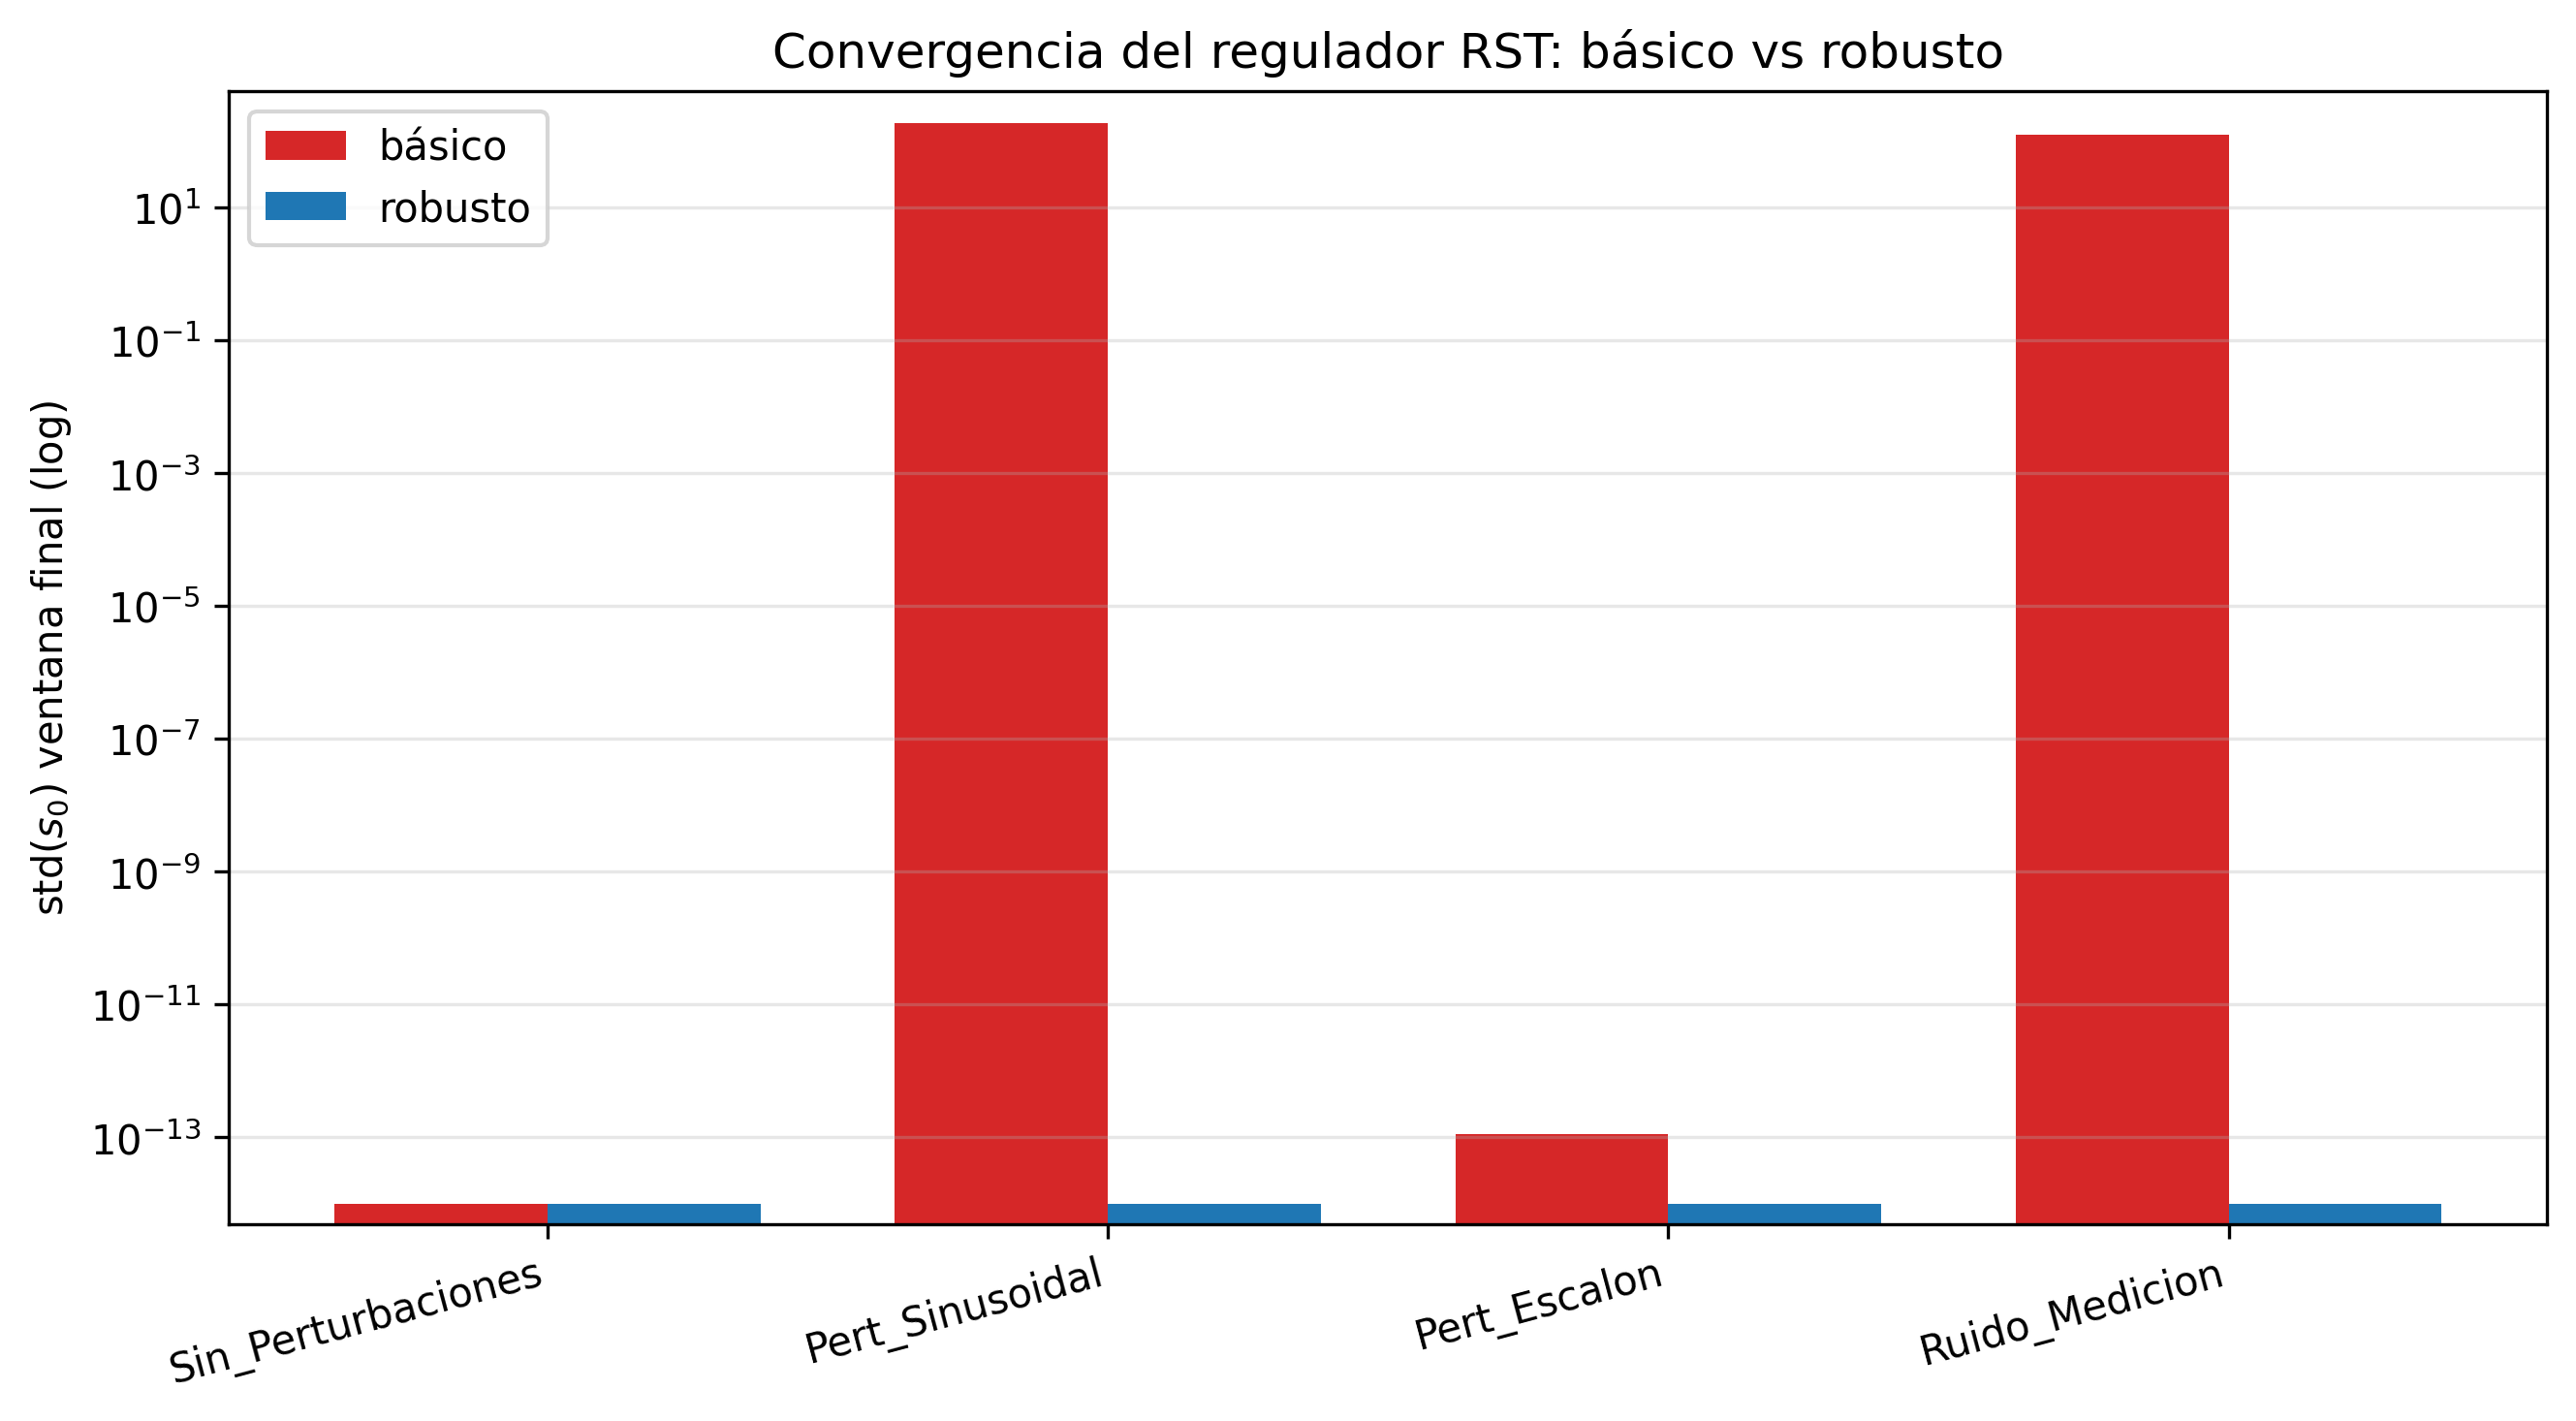
\includegraphics[width=\textwidth]{imagenes_pid_autotunning/str_convergencia.png}
\end{column}
\begin{column}{0.5\textwidth}
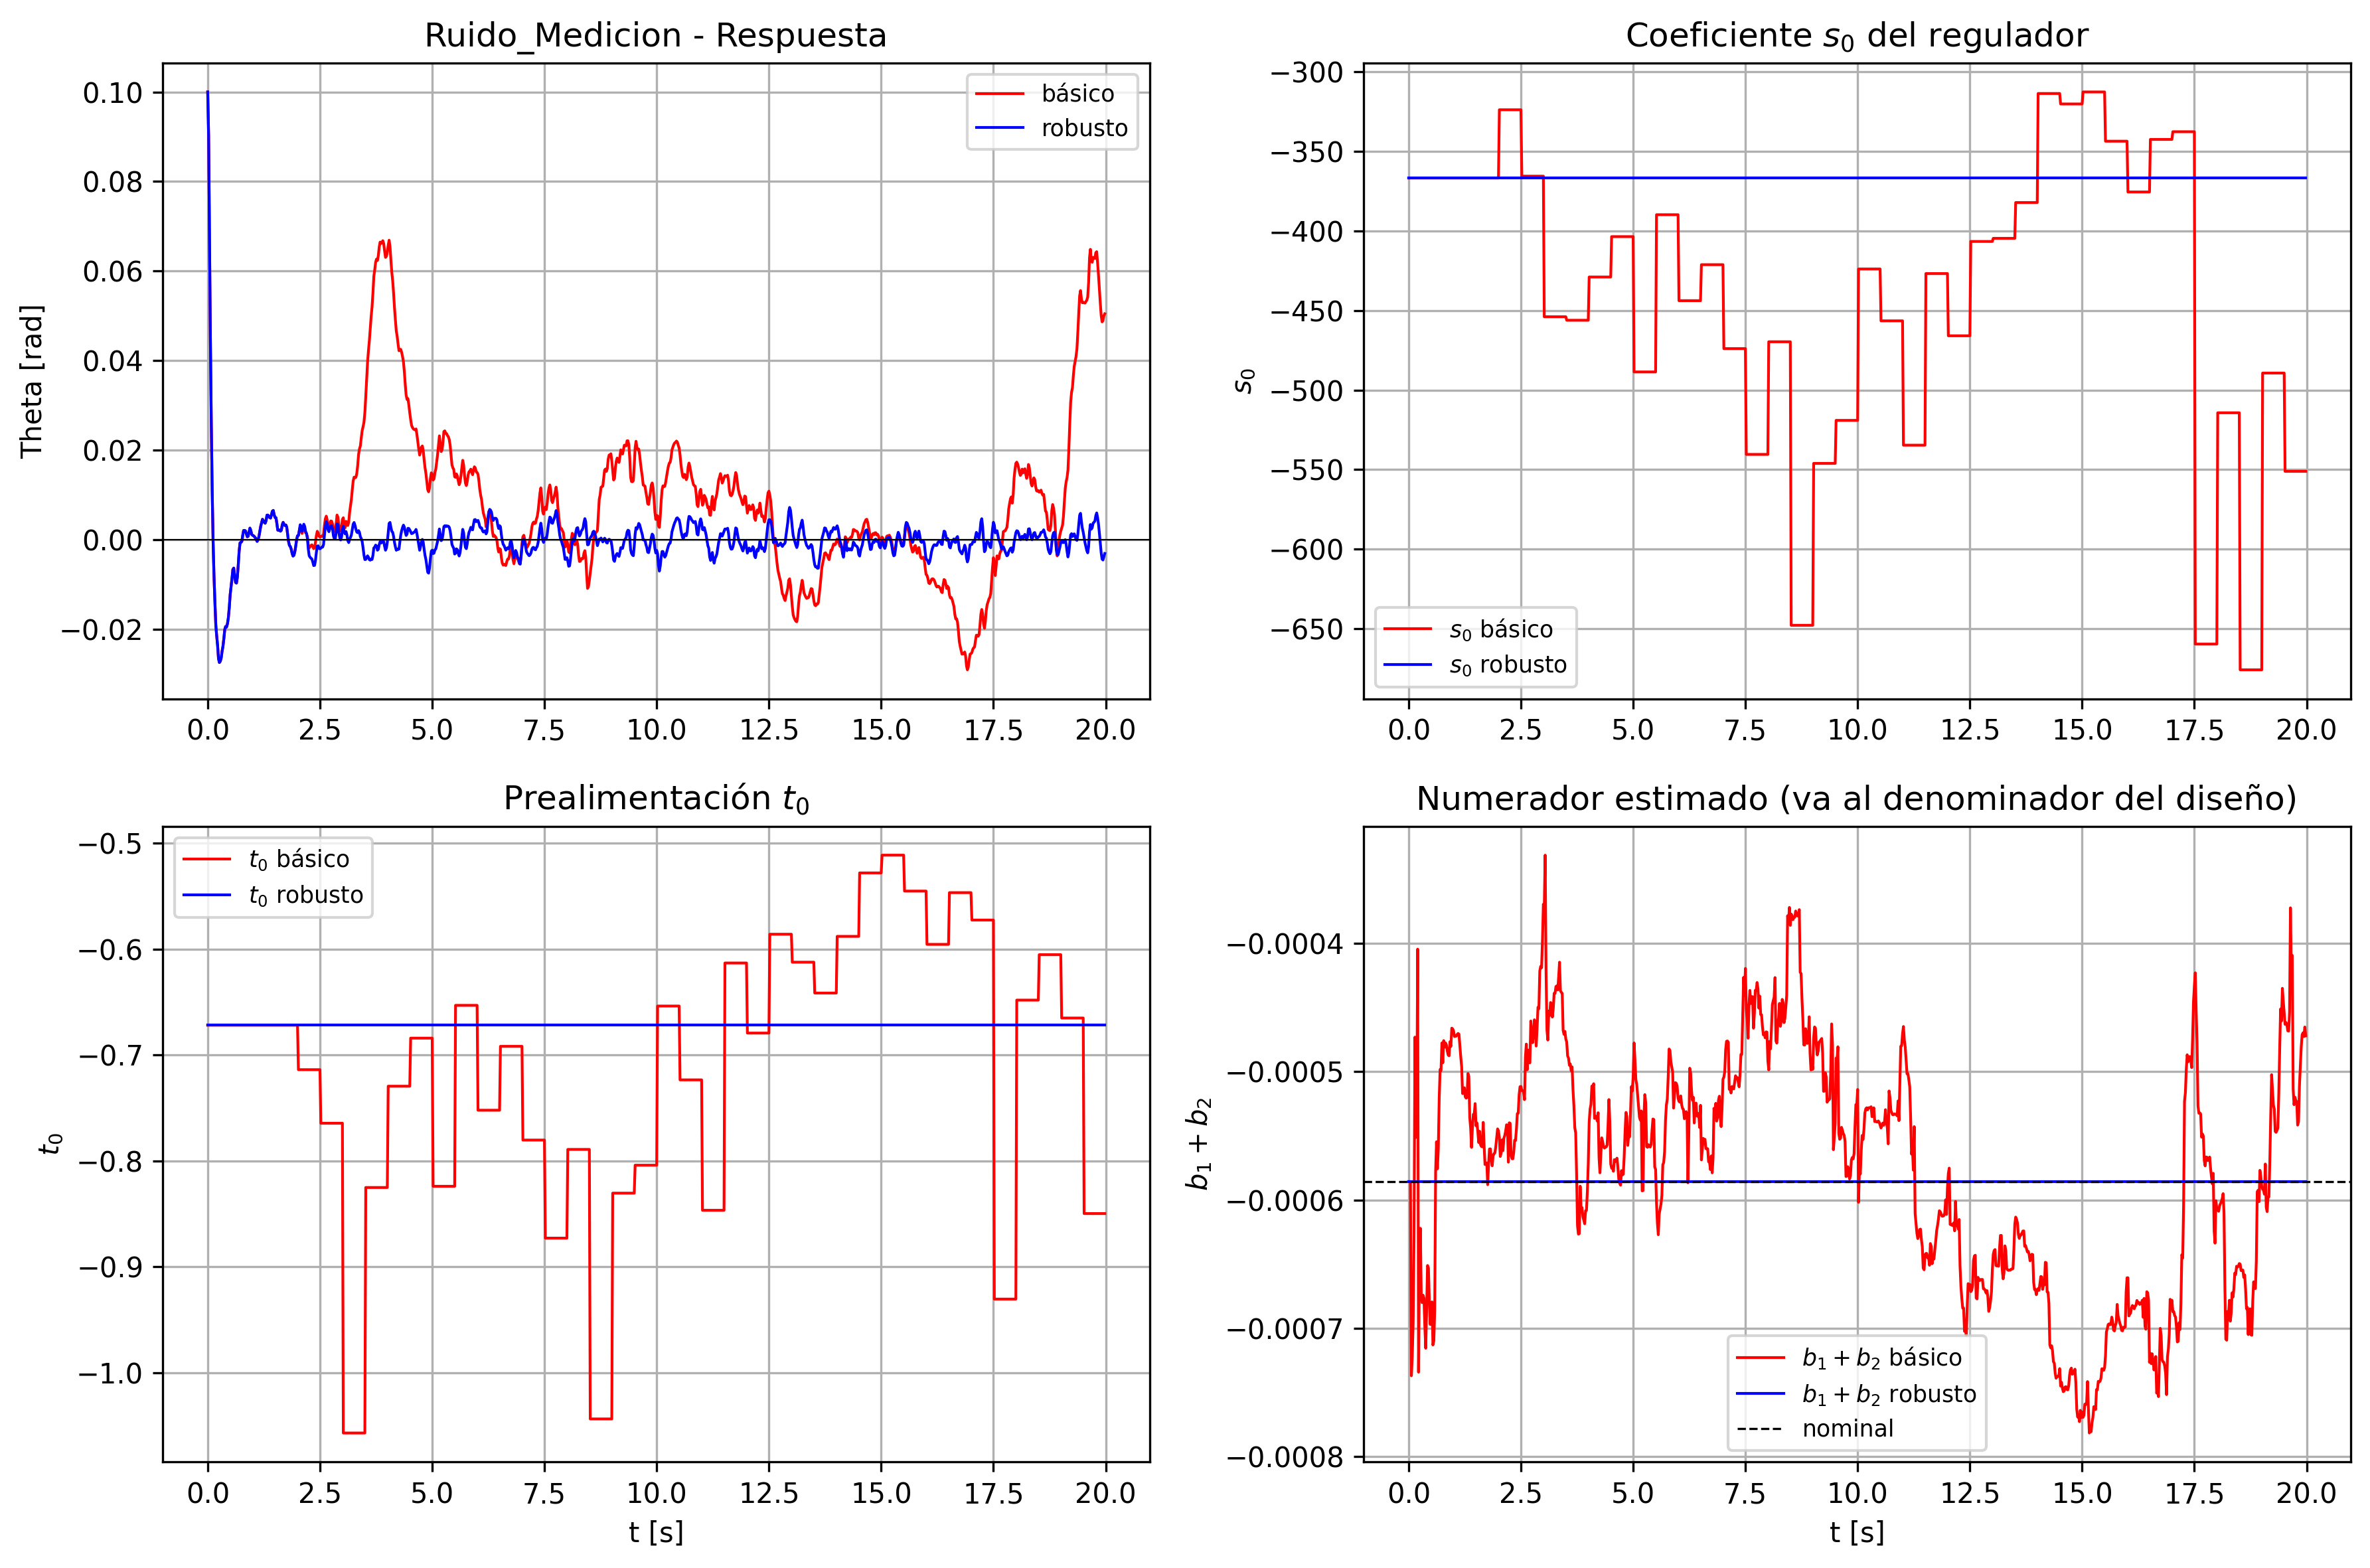
\includegraphics[width=\textwidth]{imagenes_pid_autotunning/str_cmp_Ruido_Medicion.png}
\end{column}
\end{columns}
\centering \small Básico (rojo) deriva; robusto (azul) converge. Validado con
\texttt{test\_str\_pendulo.py} (todos los tests pasan).
\end{frame}

% ==================================================================
\section{Conclusiones}
% ==================================================================

\begin{frame}{Conclusiones}
\begin{itemize}
  \item Se implementó un STR adaptativo indirecto \textbf{100\% discreto} que
  estabiliza el péndulo invertido inestable.
  \item Estimación RLS + ecuación Diofantina (Sylvester) + ley RST, con
  integrador y sin cancelar el cero no de fase mínima.
  \item Validado en 4 escenarios y con una suite de tests automáticos.
  \item El lazo es estable siempre, pero $R,S,T$ solo convergen con la
  \textbf{variante robusta} (zona muerta + gate + anti-windup): recupera los
  polos de diseño ($0{,}9418$) con ruido y perturbaciones.
  \item \textbf{Self-tuning}: el regulador converge al que se diseñaría
  conociendo la planta.
  \item Clave práctica: numerador diminuto en el denominador del diseño $\Rightarrow$
  hay que proteger la estimación (persistencia de excitación, zona muerta, gate).
\end{itemize}
\end{frame}

\end{document}
